\chapter{Objektorientierte Analyse und Entwurf}
\section{Objektorientierte Analyse}
In der objektorientierten Analyse werden die statischen und dynamischen Modelle beschrieben. Das statische Modell umfasst ein Komponentendiagramm, durch das der Aufbau und die Struktur des Projekts dargestellt werden (siehe Abb. \ref{fig:Komponentendiagramm}). Die dynamischen Modelle umfassen zwei Sequenzdiagramme. Das erste Sequenzdiagramm verdeutlicht wie die Verbindung zwischen den einzelnen Komponenten (Ultraschallgerät und mobiles Endgerät) hergestellt wird und in welcher Art und Weise die Daten übertragen werden (siehe Abb.\ref{fig:SD_Datenuebertragung}). Das zweite Sequenzdiagramm umfasst den Ablauf der Datenverarbeitung innerhalb der Applikation sowie die Anzeige der Ultraschallbilder auf der Benutzeroberfläche (siehe Abb. \ref{fig:SD_Datenverarbeitung}). Die Modelle beschreiben, wie die definierten funktionalen Anforderungen der Anforderungsanalyse umgesetzt werden können. 
\subsection{Statisches Modell}
Das folgende abgebildete Komponentendiagramm \ref{fig:Komponentendiagramm} zeigt, welche Komponenten in dem Projekt verwendet werden und welche Verbindung zwischen ihnen besteht bzw. über welche Schnittstellen diese miteinander interagieren. Die  einzelnen Komponenten sind in Subsysteme unterteilt, in denen die spezifischen Verarbeitungsschritte durchgeführt werden.  Die Komponente Sonoscape bezeichnet das Ultraschallgerät, das in die Subsysteme „Screenrecorder“, „Frame Conversion“, „Image Compression“ und den „Stream Writer\grqq unterteilt ist. Innerhalb des „Screenrecorders“ werden kontinuierlich die Ultraschallbilder des Ultraschallgeräts extrahiert bzw. Screenshots des Displays gemacht. Anschließend werden die Bilddaten durch die „Frame Conversion“ in ein entsprechendes Format konvertiert. Innerhalb des Subsystems „Image Compression“ werden die Bilddaten komprimiert. Der „Stream Writer“ überträgt die komprimierten Daten anschließend über eine TCP-IP Verbindung an die angeschlossene Netzwerkkomponente (Router/ WLAN-Stick) und durch die Verwendung einer IO-Schnittstelle weiter an das mobile Endgerät. Das mobile Endgerät umfasst die Subsysteme „Network Client“, „Stream Reader“, „data decompression“, „Frame encryption“, „Frame Processing\grqq und den „Frame Viewer“. Innerhalb des „Network Client“ wird eine Verbindung zum Ultraschallgerät aufgebaut, über die die eingehenden Daten durch den „Stream Reader“ gelesen werden. Die eingehenden Daten werden anschließend durch die „data decompression\grqq und die „Frame encryption“ dekomprimiert und  decodiert. Durch diesen Vorgang wird aus dem Rohdaten-Stream wieder ein Frame erstellt. Dieses wird in dem Subsystem „Frame Processing“ verarbeitet und die relevanten Informationen aus dem Ursprungs-Ultraschallbild ausgeschnitten und zu einem finalen Bild zusammengesetzt. Das zusammengesetzte Bild wird anschließend auf der Benutzeroberfläche bzw. dem Display des mobilen Endgerätes angezeigt. \\

\begin{figure}[H] 
\centering
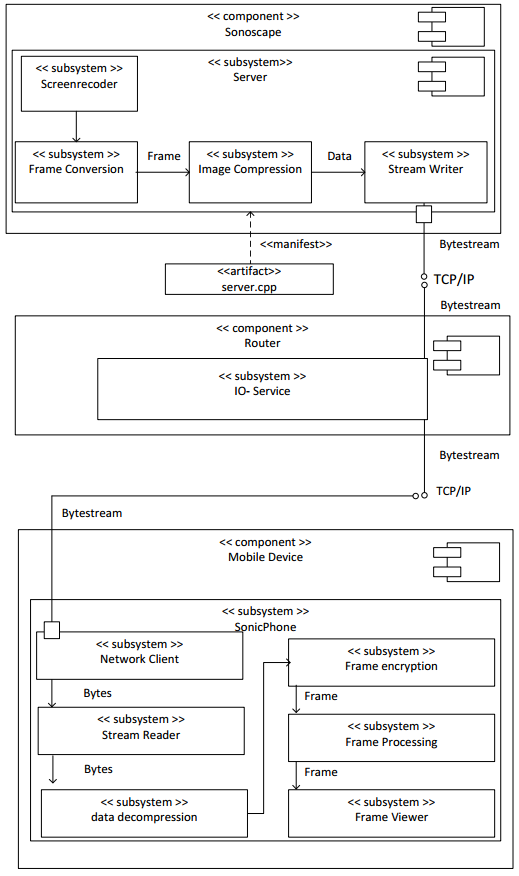
\includegraphics[width=1\textwidth, height = 1\textheight]{Bilder/objektorientierteAnalyseundEntwurf/KD_Komponentendiagramm}
\caption{{\small Komponentendiagramm des gesamten Systems}}
\label{fig:Komponentendiagramm}
\end{figure}

\subsection{Dynamisches Modell}
Die folgenden zwei Sequenzdiagramme \ref{fig:SD_Datenuebertragung} und \ref{fig:SD_Datenverarbeitung}  verdeutlichen den Ablauf des Verbindungsaufbaus zwischen Ultraschallgerät und mobilem Endgerät sowie die \\ Übertragung der Ultraschallbilder.\\
Die Datenübertragung wird durch die Implementierung eines Servers auf dem Ultraschallgerät durchgeführt. Durch den Einsatz eines IO-Services und einem erzeugten TCP-Socket werden die Ultraschallbilder in Form eines Bytestream zwischen Ultraschallgerät und mobilen Endgerät übertragen. Zuerst werden die Ultraschallaufnahmen durch kontinuierliche Screenshots aufgenommen. Anschließend werden diese in RGB konvertiert und durch einen Algorithmus komprimiert. Nach der Verarbeitung der Daten auf der Serverseite werden die Daten über einen Bytestream übertragen. Für den Verbindungsaufbau wird auf der Serverseite ein Socket erstellt, welches an eine Adresse (Port) gebunden wird. Dadurch können Anfragen zum Verbindungsaufbau akzeptiert werden. Ein entsprechender Serverprozess „lauscht“ dann an dem Port auf Verbindungsanfragen (listen). Bei einer einkommenden Verbindungsanfrage wird daraufhin ein Kommunikationssocket (accept) erzeugt. Die aufgebaute Verbindung wird nun für die Kommunikation und die Datenübertragung zwischen dem Ultraschallgerät und dem mobilen Endgerät genutzt. Die Verbindung bleibt solange bestehen bis eine der beiden Seiten die Verbindung beendet. 

\begin{figure}[H] 
\centering
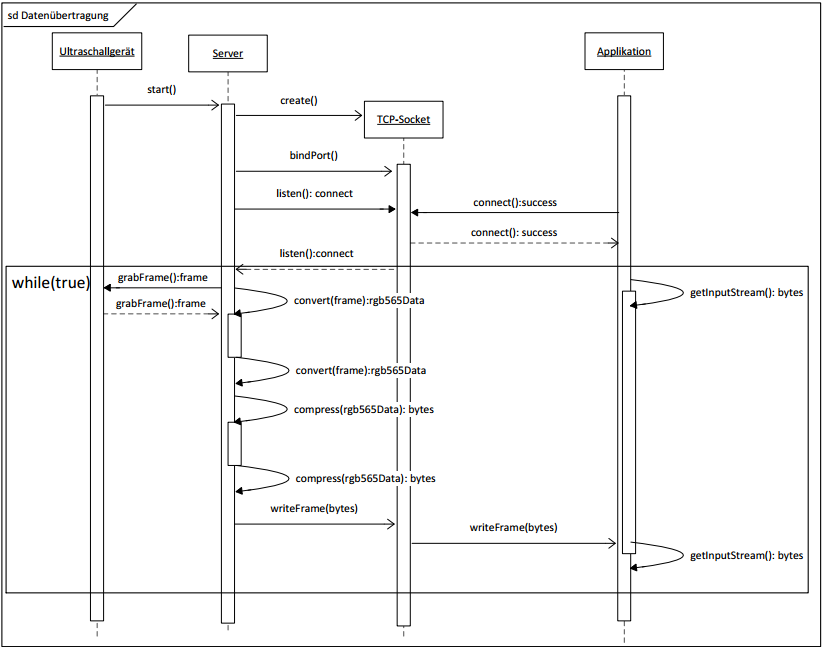
\includegraphics[width=1\textwidth]{Bilder/objektorientierteAnalyseundEntwurf/SD_Datenuebertragung}
\caption{{\small Datenübertragung zw. Ultraschallgerät und der mobilen Applikation}}
\label{fig:SD_Datenuebertragung}
\end{figure}

Das folgende Sequenzdiagramm \ref{fig:SD_Datenverarbeitung} veranschaulicht die notwendigen Schritte für einen Verbindungsaufbau durch die Clientseite (mobiles Endgerät) und den Datenverarbeitungsprozess der Ultraschallbilder. Für den Verbindungsaufbau wird auf dem Client ein Socket erstellt und mit dem Server (über die IP-Adresse) eine Verbindung aufgebaut (connect). Über diese Verbindung werden anschließend die Daten angefordert. Der Client verbindet sich dafür mit dem Kommunikationssocket und sendet und empfängt Daten. Der übertragende Bytestream wird in der Applikation empfangen, dekomprimiert und die einzelnen Bilder (Bitmaps) werden extrahiert. Aus dem extrahierten Bild werden anschließend über drei verschiedene Funktionen das Ultraschallbild, die Farbskala und eine Liste von Informationen (bspw. FPS etc.) ausgeschnitten und zu einem neuen Bild zusammengesetzt. Das erzeugte Bild wird dann auf der Benutzeroberfläche angezeigt und anschließend wieder gelöscht und der belegte Speicherplatz freigegeben. Abschließend wird die Verbindung zum Server auf dem Ultraschallgerät getrennt und das Socket geschlossen.

\begin{figure}[H] 
\centering
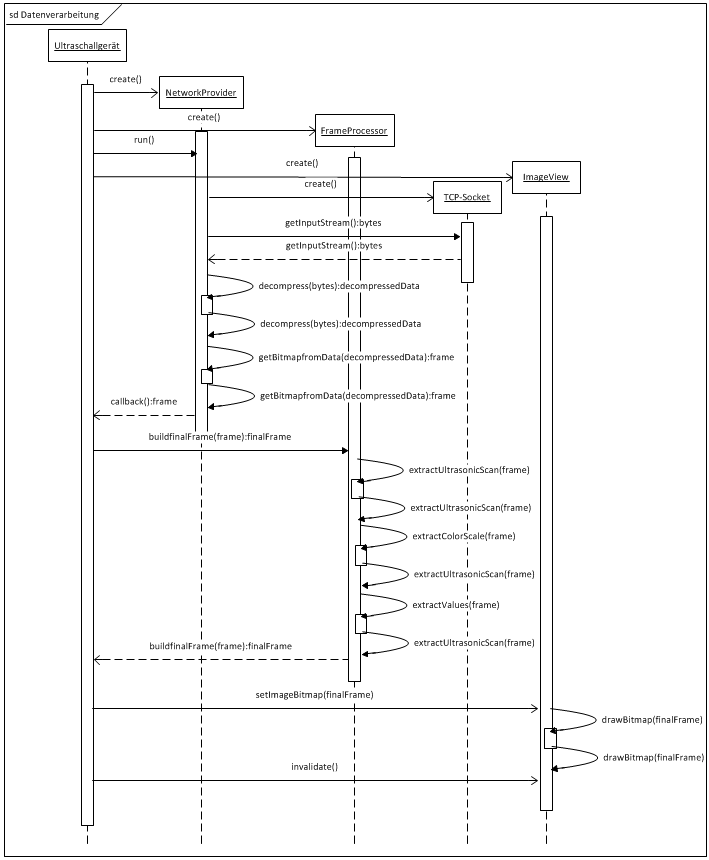
\includegraphics[width=1\textwidth]{Bilder/objektorientierteAnalyseundEntwurf/SD_Datenverarbeitung}
\caption{{\small Datenverarbeitung in der mobilen Applikation}}
\label{fig:SD_Datenverarbeitung}
\end{figure}

\section{Objektorientierter Entwurf}
Die Überführung der Ergebnisse der objektorientierten Analyse in den  objektorientierten Entwurf werden dafür verwendet eine konkrete Softwarearchitektur zu erstellen, die als direkte Implementierungsvorlage dient. Im Folgenden wird die Softwarearchitektur in Form eines Klassendiagramms dargestellt. Da das Betriebssystem des Smartphone LG G4 das Android Betriebsystem der Version 5.1 ist (vgl. Abschnitt \ref{LGG4}), wird die mobile Applikation unter Verwendung des Android SDKs (vgl. Abschnitt \ref{Android}) in der Programmiersprache Java implementiert.  \\
Das nachfolgend abgebildete Klassendiagramm \ref{fig:cd_mobileApplikation} beschreibt sämtliche Klassen und deren Beziehungen untereinander, die angelegt werden, um die mobile Applikation zu realisieren. Aus Rücksicht auf die Übersichtlichkeit wurde auf die Abbildung sämtlicher Get- und Set- Methoden verzichtet. In der Klasse \grqq MainActivity\grqq werden die Objekte für die Klassen \grqq NetworkProvider \grqq und \grqq FrameProcessorImpl\grqq \linebreak instanziiert. Die \grqq NetworkProvider\grqq -Klasse erbt die Attribute und Funktionen des Interfaces \grqq IFrame"-Providers\grqq und wird um die benötigten Funktionen für den Verbindungsaufbau zum Server (Ultraschallgerät) erweitert. Die \grqq FrameProcessorImpl\grqq - Klasse erbt von dem Interface \grqq IFrameProcessor\grqq und erweitert die Funktionalität für den Verarbeitungsprozess der übertragenen Ultraschallbilder. Zur Anzeige der Ultraschallbilder auf der Benutzeroberfläche wurde das vordefinierte \grqq ImageView\grqq -Widget der Android- API um entsprechende Listener-Methoden erweitert, die eine Eventbehandlung bei Änderungen des \grqq ImageViews\grqq ermöglichen. Hierdurch kann das \grqq ImageView\grqq  für eine kontinuierliche Darstellung und anschließende Entfernung sowie Freigabe des benötigten Speicherplatzes der Ultraschallbilder durch eine entsprechende Aktualisierung verwendet werden.  

\begin{figure}[H] 
\centering
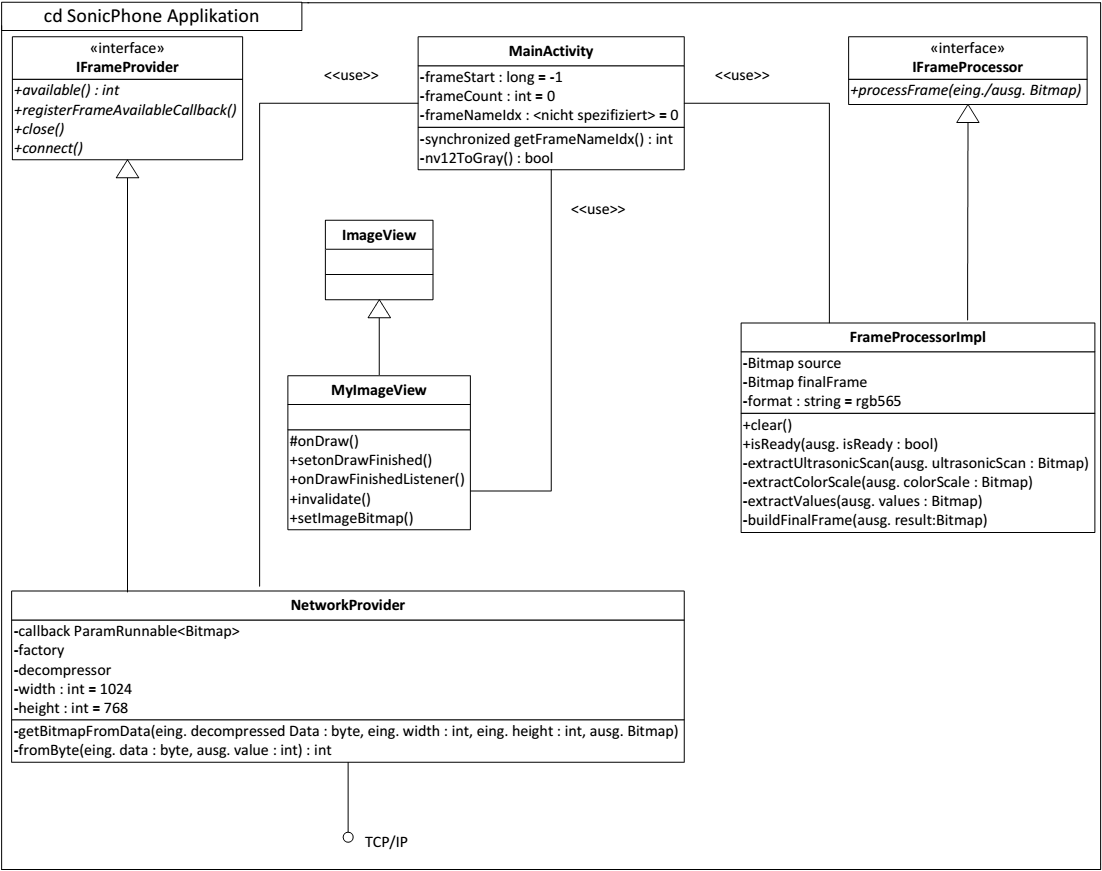
\includegraphics[width=1\textwidth]{Bilder/objektorientierteAnalyseundEntwurf/cd_mobileApplikation}
\caption{{\small Klassendiagramm der mobilen Applikation}}
\label{fig:cd_mobileApplikation}
\end{figure}
